\documentclass[12pt,a4paper,openright,twoside]{report}
\usepackage[italian,english]{babel}
\usepackage{fancyhdr}
\usepackage{indentfirst}
\usepackage{newlfont}
\usepackage{pdfpages}
\usepackage{abstract}
\oddsidemargin=30pt \evensidemargin=20pt
\pagestyle{fancy}\addtolength{\headwidth}{20pt}\setlength{\headheight}{15pt}
\renewcommand{\chaptermark}[1]{\markboth{\thechapter.\ #1}{}}
\renewcommand{\sectionmark}[1]{\markright{\thesection \ #1}{}}
\rhead[\fancyplain{}{\bfseries\leftmark}]{\fancyplain{}{\bfseries\thepage}}
\cfoot{}
\linespread{1.3}
\begin{document}
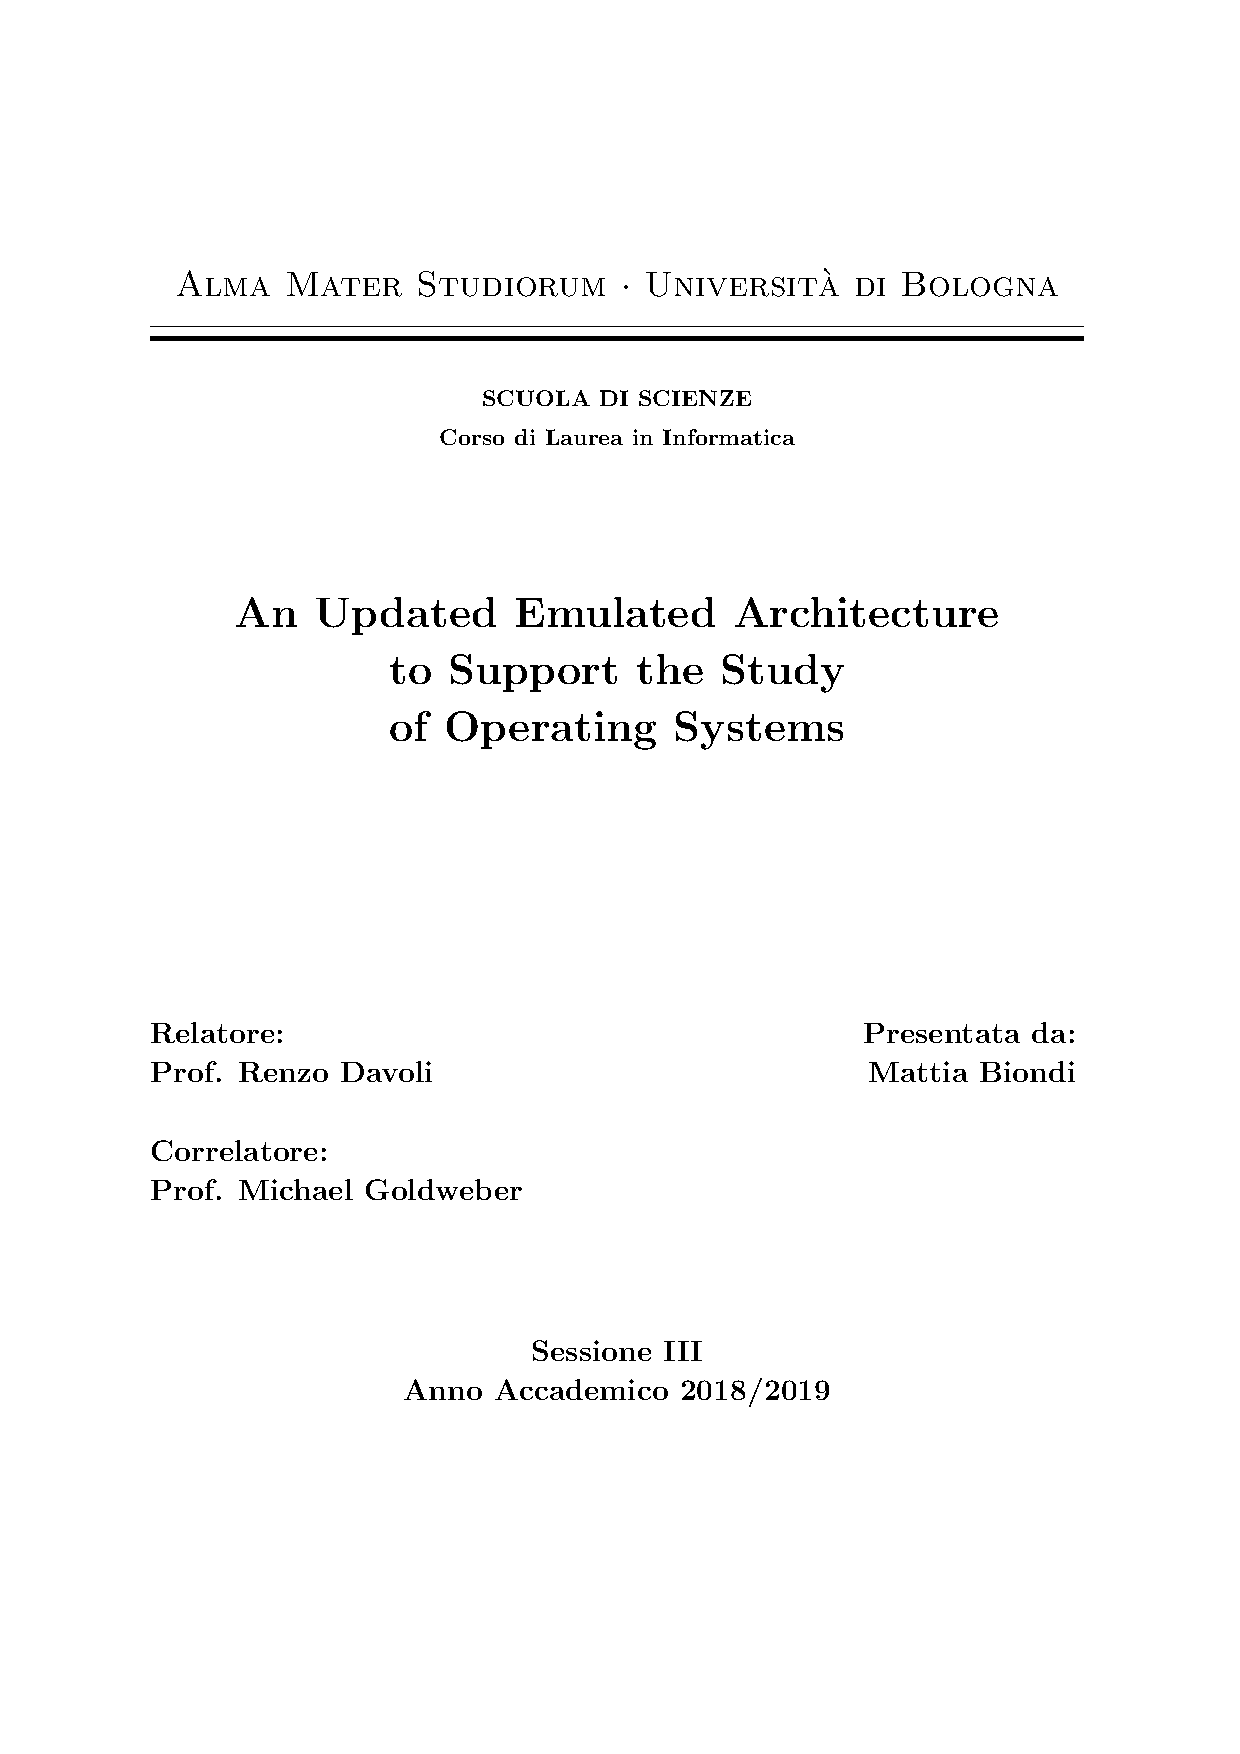
\includepdf[pages=-]{titlepage.pdf}
\clearpage{\pagestyle{empty}\cleardoublepage}
\begin{titlepage}
	\thispagestyle{empty}
	\topmargin=6.5cm
	\raggedleft
	\large
	\em
	dedica
	
	\newpage
	\clearpage{\pagestyle{empty}\cleardoublepage}
\end{titlepage}
\begin{abstract}
	One of the most effective ways to learn something new is by actively practising it, and there is---maybe---no better way to study an Operating Systems course than by building your OS.
	
	However, it is important to emphasize how the realization of an operating system capable of running on a real hardware machine could be an overly complex and unsuitable task for an undergraduate student.
	Nonetheless, it is possible to use a simplified computer system simulator to achieve the goal of teaching Computer Science foundations in the university environment, thus allowing students to experience a quite realistic representation of an operating system.
	
	$\mu$MPS has been created for this purpose, a pedagogically appropriate machine emulator, based around the MIPS R2/3000 microprocessor, which features an accessible architecture that includes a rich set of easily programmable devices.
	$\mu$MPS has an almost two decades old historical development and the outcome of this following thesis is the third version of the software, dubbed $\mu$MPS3.
	This second major revision aims to simplify, even more, the emulator’s complexity in order to lighten the load of work required by the students during the OS design and implementation.
	Two of these simplifications are the removal of the virtual memory bit, which allowed address translation to be turned on and off, and the replacement of the tape device, used as storage devices, with a new flash drive device---certainly something more familiar to the new generation of students.

	Thanks to the employment of this software and the feed-backs received over the last decade, it has been possible to realize not just this following thesis, but also to develop some major improvements, which concern everything from the project building tools to the front-end, making $\mu$MPS a modern and reliable educational software.
\end{abstract}
\clearpage{\pagestyle{empty}\cleardoublepage}
\tableofcontents
\addtocontents{toc}{\protect\thispagestyle{empty}}
\thispagestyle{empty}
\clearpage{\pagestyle{empty}\cleardoublepage}
\pagenumbering{arabic}
\chapter{Introduction}
\lhead[\fancyplain{}{\bfseries\thepage}]{\fancyplain{}{\bfseries\rightmark}}

\section{Background}
	The study and the consequent implementation of how an operating system works is, by now, a long-established and consolidated practice in every Computer Science's curriculum.
	It is, actually, one of the crucial components of a computer and it is responsible of ensuring it's basic operations, by coordinating and managing the system's resources like processor, memory, devices and processes, thus allowing hardware and software to interface each other.
	
	This is probably the first real example of ``big project'' which students must experience, thanks to complex intercommunication system that has to exist between the different machine's components, and the study of it allows to comprehend the most common software engineering practices.
	
	The approach on practical contexts is essential to fully understand how a machine works behind the theoretical notions studied in the early stages of the course of study, and it is usually followed by the debate of which is the best teaching choice concerning processor architectures.
	
	Obviously, there is not only one way of how a central processor unit can be implemented, and while older realizations---although applicable for educational purposes---are now obsolete and incompatible with current platforms, modern ones are designed to achieve high speed and quality, which makes them overly complex and unsuitable for the pedagogic experience.
	
	Over the years, the MIPS architecture has become one of the landmarks in this teaching choice due to its clean and elegant instruction set, despite being excessively convoluted to student’s perception, because of the high level of details obscuring the basic underlying features of it.
	A potential solution to this problem is the adoption of a simplified computer system simulator, like $\mu$MPS, to bring together an adequate level of understanding and a realistic representation of a real operating system.

\section{History of $\mu$MPS}
	$\mu$MPS is based on the machine emulator MPS \cite{mps}, designed and realized by Professor Renzo Davoli and one of his graduate students Mauro Morsiani, in the late 1990s at the University of Bologna.
	
	The initial purpose was to bring back to life the layout and implementation experience of an operating system through an educational emulator, which could be run on real hardware.
	This practice was already possible in the past years, when the processor's architecture studied were the same available on real machines, but it has gone lost through the years because of the high-speed development of new more complex technologies used on physical implementations.
	
	MPS was able to emulate the MIPS R3000 processor along with five other different device categories: disks, tapes, network adapters, printers and terminals.
	
	The concerned CPU was genuinely emulated together with its complex virtual memory management system, which was the main subject of the feed-backs received during class testing of MPS as a pedagogical tool at the University of Bologna and Xavier University, in an undergraduate operating systems courses, taught respectively by Renzo Davoli and Michael Goldweber.
	
	It was tested through \textit{Kaya}'s \cite{kaya} implementation, one of the variety of graduate-level projects that the emulator can support.
	
	The urge of simplification led to the creation of $\mu$MPS, virtually identical to MPS but with the addition of a virtual memory management subsystem which had to resemble as much as possible to the conceptual one found in popular introductory OS texts.
	The only other difference was the new novice-friendly graphical user interface, significantly improved again in 2011 by Tomislav Jonjic during the development of the first major revision of the emulator, $\mu$MPS2 \cite{umps2}, which also implemented the support to up to sixteen MIPS R3000-style processors.

\section{$\mu$MPS3}
	More than ten years have passed since the first release of $\mu$MPS and as many have passed from the moment it has been developed into a consolidated educational tool in the two already acknowledged teaching courses.
	
	As already mentioned, the students' observations during this period were essential to in-depth testing the $\mu$MPS emulator as a pedagogical tool, showing as a result that further changes were needed.
	Some examples of these modifications would be the memory's structure and management system of both physical and virtual ones, a nuance probably still too complex and confusing, which could feel like a regression, since the attempt to simplify it has led to the removal of the VM bit.
	This was originally introduced in the first version of $\mu$MPS, as a distinctive feature from its predecessor MPS.
	On the other hand, other changes are related to the passage of the years, such as the replacement of memory tapes with flash drive devices, also know as ``USB sticks'' or ``SD cards''.
	
	Tapes are probably still studied in their operation nowadays, but they cannot be found in today's practical contexts, and therefore it could be difficult to understand for the new generation of students, who can't find a match in current technological implementations.
	
	Another consequence of $\mu$MPS's modernization has been the shift from the historical and well established Autotools to a more modern building tool, CMake, that speeds up the compilation process in addition to simplify the project's structure.
	It also fits best with the current emulator's graphical user interface, originally built upon Qt4, which also undergoes to the migration to the new version, Qt5.
	
	These and more changes are collected together in a major release of the project, $\mu$MPS3, consequently bringing even more reliability in terms of pedagogical tool.
	
	Due to implementation aspects---unlike his predecessor $\mu$MPS2---this new version is not backward compatible with older ones.

	\texttt{here I could talk about the Debian Packaging I will do when everything is finalized}
\section{Document's Structure}
\chapter{Memory Management}
\lhead[\fancyplain{}{\bfseries\thepage}]{\fancyplain{}{\bfseries\rightmark}}
	As for the two prior versions, the memory subsystem of $\mu$MPS3 is divided into physical and virtual, and both have undergone significant changes in this major revision.
	The main reasons for the modifications made are the further simplification of the work required by the user for the kernel implementation and the better clarification of the emulator's memory internal view which caused some confusion during the more than 10 years of use of $\mu$MPS as an educational tool in operating system courses.

\section{Physical Memory}
	The physical address space is divided into two big areas: a kernel reserved space, from address \texttt{0x0000.0000} to \texttt{0x1FFF.FFFF}, and the installed RAM, from address \texttt{0x2000.0000} to \texttt{RAMTOP}.
	This last value is calculated upon the value retrieved from the configuration file, settable from the machine config dialog in the front-end emulator, which goes from a minimum of 8 to a maximum of 512 memory frames.
	Being the size of every frame 4 kilobyte, $\mu$MPS can have from 32KB up top 2MB of installed RAM. Hence, the value of \texttt{RAMTOP} range from \texttt{0x2000.8000} to \texttt{0x2020.0000}.

	The first area was reserved for:
	\begin{itemize}  
	\item Execution ROM code, which layed in a read-only segment from address \texttt{0x0000.0000} to \texttt{ROMTOP};
	\item prova.
	\end{itemize}
	This address space, corresponding to the first 0.5GB of physical memory, causes the raising of an Address Error when trying to access it while the processor was in user-mode.
\section{TLB Floor Address}
\section{VM Bit Removal}
\chapter{Exception Handling}
\lhead[\fancyplain{}{\bfseries\thepage}]{\fancyplain{}{\bfseries\rightmark}}
\section{Primary Design}
\section{BIOS Data area}
\lhead[\fancyplain{}{\bfseries\thepage}]{\fancyplain{}{\bfseries\rightmark}}
\chapter{Flash Devices}
\lhead[\fancyplain{}{\bfseries\thepage}]{\fancyplain{}{\bfseries\rightmark}}
\section{Tape Readers}
\section{Flash Drives}
\chapter{Project Modernization}
\lhead[\fancyplain{}{\bfseries\thepage}]{\fancyplain{}{\bfseries\rightmark}}
\section{CMake Migration}
\section{Qt5 Transition}
\section{Logo and Icon Theme}
\chapter{Linux Packaging}
\lhead[\fancyplain{}{\bfseries\thepage}]{\fancyplain{}{\bfseries\rightmark}}
\section{Debian Package}
\section{Arch Linux Package}
\chapter{Conclusions}
\lhead[\fancyplain{}{\bfseries\thepage}]{\fancyplain{}{\bfseries\rightmark}}
	Knowing how an operating system works should be common knowledge and not something restricted only to the ones who studied in the IT field.
	If you are reading this document there are high chances you are doing it on a device of your property, which is running an operating system, and you should know how all of this really works in other to really feel like you own this particular system.
\begin{thebibliography}{99}
	\addcontentsline{toc}{chapter}{Bibliography}

	\bibitem{mps}
	M. Morsiani, R. Davoli,
	\textit{Learning Operating Systems Structure and Implementation through the MPS Computer System Simulator},
	in \textit{The Proceedings of the Thirtieth SIGCSE Technical Symposium on Computer Science Education},
	SIGCSE ’99, (New York, NY, USA), pp. 63-67, ACM, March 1999.

	\bibitem{kaya}
	M. Goldweber, R. Davoli, and M. Morsiani,
	\textit{The Kaya OS Project and the $\mu$MPS Hardware Emulator},
	in \textit{Proceedings of the 10th Annual SIGCSE Conference on Innovation and Technology in Computer Science Education},
	ITiCSE ’05, (New York, NY, USA), pp. 49–53, ACM, June 2005.
	
	\bibitem{umps2}
	M. Goldweber, R. Davoli, and T. Jonjic,
	\textit{Supporting Operating Systems Projects Using the $\mu$MPS2 Hardware Simulator},
	in \textit{Proceedings of the 17th ACM Annual Conference on Innovation and Technology in Computer Science Education},
	ITiCSE ’12, (New York, NY, USA), pp. 63–68, ACM, July 2012.

\end{thebibliography}
\end{document}
